\documentclass[main.tex]{subfiles}
\begin{document}

\chapter{Maximum Likelihood and the Invariance Principle}\label{ch:mle}\chaptermark{Maximum Likelihood and Invariance}

The unbiased estimation theory of the previous chapters is elegant but not applicable to every problem: a complete sufficient statistic\index{complete statistic@complete statistic}\index{sufficient statistic@sufficient statistic} may not exist, and an unbiased estimator\index{unbiased estimator@unbiased estimator} may not exist. Fisher's maximum likelihood\index{maximum likelihood estimator mle@maximum likelihood estimator (MLE)} (ML) principle, by contrast, offers an almost universal recipe: choose the parameter value that makes the observed data ``most likely''. ML estimators are usually biased, but in large samples they are consistent, asymptotically normal\index{asymptotic normality@asymptotic normality} and efficient (Chapter~\ref{ch:mle-asimptotik}). In this chapter we discuss the definition of the MLE, its computation, its invariance property and its pitfalls.

\section{Definitions}

\begin{definition}[Likelihood and Log-Likelihood]
After $\x$ has been observed, the function $\theta\mapsto L(\theta;\x)=f(\x;\theta)$ is called the \emph{likelihood function\index{likelihood function@likelihood function}} and $\ell(\theta;\x)=\ln L(\theta;\x)$ the \emph{log-likelihood\index{log likelihood@log-likelihood}}. For an i.i.d.\ sample, $L(\theta;\x)=\prod_{i=1}^nf(x_i;\theta)$ and $\ell(\theta;\x)=\sum_{i=1}^n\ln f(x_i;\theta)$.
\end{definition}

\begin{remark}
The likelihood is a function of $\theta$ and is \emph{not} a probability distribution on $\theta$: $\int L(\theta;\x)d\theta$ is generally not $1$. Only its ratios are meaningful; $L(\theta_1;\x)/L(\theta_2;\x)$ measures how much the data support $\theta_1$ relative to $\theta_2$ (the likelihood principle).
\end{remark}

\begin{definition}[Maximum Likelihood Estimator --- MLE]\index{maximum likelihood estimator mle@maximum likelihood estimator (MLE)|textbf}
A statistic $\hat\theta(\X)$ satisfying, for every $\x$,
\[
L(\hat\theta(\x);\x)=\sup_{\theta\in\Theta}L(\theta;\x)
\]
is called the \emph{maximum likelihood estimator} (MLE) of $\theta$. If $\ell$ is differentiable and the maximum is at an interior point of $\Theta$, the MLE is a solution of the \emph{likelihood equations} $\nabla_\theta\ell(\theta;\x)=\mathbf 0$.
\end{definition}

\begin{definition}[Induced (Profile) Likelihood]\label{def:induklenmis}
Let $g:\Theta\to\Lambda$ be a function, not necessarily one-to-one. For $\eta\in\Lambda$ the function
\[
L^*(\eta;\x)=\sup_{\{\theta:\,g(\theta)=\eta\}}L(\theta;\x)
\]
is called the \emph{induced likelihood\index{profile likelihood@profile likelihood}}. The $\hat\eta$ maximising $L^*$ is called the MLE of $g(\theta)$.
\end{definition}

\section{Main Theorems and Proofs}

\begin{theorem}[Zehna's Invariance Principle \cite{zehna66}]\label{thm:zehna}\index{zehna s invariance principle@Zehna's invariance principle}
If $\hat{\theta}$ is the MLE of $\theta$, then for \emph{any} function $g$ the MLE of $g(\theta)$ is $g(\hat{\theta})$:
\[
\widehat{g(\theta)}_{\text{MLE}} = g(\hat{\theta}_{\text{MLE}}).
\]
\end{theorem}
\begin{proof}
Let $\hat\eta=g(\hat\theta)$. For every $\eta\in\Lambda$,
\[
L^*(\eta;\x)=\sup_{\theta:g(\theta)=\eta}L(\theta;\x)\le\sup_{\theta\in\Theta}L(\theta;\x)=L(\hat\theta;\x).
\]
On the other hand, since $\hat\theta$ belongs to $\{\theta:g(\theta)=\hat\eta\}$, $L(\hat\theta;\x)\le L^*(\hat\eta;\x)$. Combining the two inequalities, $L^*(\eta;\x)\le L^*(\hat\eta;\x)$ for every $\eta$; i.e.\ $\hat\eta=g(\hat\theta)$ maximises $L^*$.
\end{proof}

\begin{remark}
Invariance is a property that unbiasedness \emph{lacks}: $S^2$ is unbiased for $\sigma^2$ while $S$ is biased for $\sigma$; but if $\hat\sigma^2$ is the MLE of $\sigma^2$, then $\hat\sigma=\sqrt{\hat\sigma^2}$ is the MLE of $\sigma$. Practical consequence: the parametrisation in which you set up a model does not change the MLE; in numerical optimisation, unconstrained parametrisations (e.g.\ $\ln\sigma$, logit) can be used freely.
\end{remark}

\begin{proposition}[The MLE Is a Function of the Sufficient Statistic]\label{prop:mle-yeterli}\index{maximum likelihood estimator mle@maximum likelihood estimator (MLE)}
If $T$ is sufficient and the MLE is unique, then $\hat\theta$ depends only on $T$.
\end{proposition}
\begin{proof}
By factorisation\index{factorisation theorem@factorisation theorem}, $L(\theta;\x)=g(T(\x),\theta)h(\x)$; the constant factor $h(\x)>0$ does not affect the maximiser, so $\hat\theta=\argmax_\theta g(T(\x),\theta)$.
\end{proof}

\begin{theorem}[The MLE in a Natural Exponential Family]\label{thm:ustel-mle}\index{maximum likelihood estimator mle@maximum likelihood estimator (MLE)}
Let the $X_i$ be i.i.d.\ from the natural-form family $f(x;\bm\eta)=h(x)\exp\{\bm\eta^\top\mathbf t(x)-A(\bm\eta)\}$ with an open natural parameter\index{natural parameter@natural parameter} space. Then $\ell(\bm\eta)=\bm\eta^\top\sum\mathbf t(x_i)-nA(\bm\eta)+\text{const}$ is strictly concave and the MLE (if it exists) is unique; the likelihood equation
\[
\nabla A(\hat{\bm\eta})=\E_{\hat{\bm\eta}}[\mathbf t(X)]=\frac1n\sum_{i=1}^n\mathbf t(X_i)
\]
takes the form ``equate theoretical moments with sample moments''.
\end{theorem}
\begin{proof}
Differentiating $e^{A(\bm\eta)}=\int h(x)e^{\bm\eta^\top\mathbf t(x)}dx$ gives $\nabla A=\E[\mathbf t(X)]$ and $\nabla^2A=\Cov(\mathbf t(X))$. Since the covariance matrix\index{covariance matrix@covariance matrix} is positive definite (for a full-rank family), $A$ is strictly convex and $\ell$ strictly concave; a strictly concave function has at most one critical point, and that point is the global maximum.
\end{proof}

% <<fig:olabilirlik>>
How the likelihood function\index{likelihood function@likelihood function} narrows as data accumulate can be seen in Figure~\ref{fig:olabilirlik}.

\begin{figure}[ht]
\centering
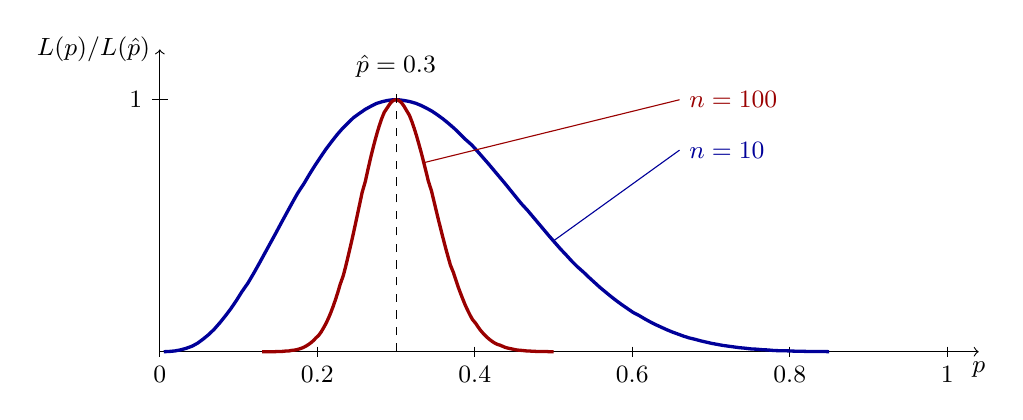
\begin{tikzpicture}[x=10cm,y=3.2cm,font=\small]
\draw[->] (0,0) -- (1.04,0) node[below] {$p$}; \draw[->] (0,0) -- (0,1.2) node[left] {$L(p)/L(\hat p)$};
\foreach \x in {0,0.2,0.4,0.6,0.8,1} \draw (\x,0.02) -- (\x,-0.02) node[below] {\x};
\draw (0.01,1) -- (-0.01,1) node[left] {1};
\draw[very thick,blue!60!black] (0.005,0.000) -- (0.012,0.001) -- (0.019,0.003) -- (0.026,0.007) -- (0.033,0.013) -- (0.041,0.022) -- (0.048,0.034) -- (0.055,0.050) -- (0.062,0.068) -- (0.069,0.089) -- (0.076,0.114) -- (0.083,0.141) -- (0.090,0.170) -- (0.097,0.202) -- (0.104,0.237) -- (0.112,0.273) -- (0.119,0.310) -- (0.126,0.349) -- (0.133,0.389) -- (0.140,0.429) -- (0.147,0.469) -- (0.154,0.510) -- (0.161,0.550) -- (0.168,0.590) -- (0.175,0.629) -- (0.183,0.667) -- (0.190,0.704) -- (0.197,0.739) -- (0.204,0.772) -- (0.211,0.804) -- (0.218,0.833) -- (0.225,0.861) -- (0.232,0.886) -- (0.239,0.908) -- (0.246,0.929) -- (0.254,0.947) -- (0.261,0.962) -- (0.268,0.974) -- (0.275,0.985) -- (0.282,0.992) -- (0.289,0.997) -- (0.296,1.000) -- (0.303,1.000) -- (0.310,0.997) -- (0.317,0.993) -- (0.325,0.986) -- (0.332,0.977) -- (0.339,0.966) -- (0.346,0.954) -- (0.353,0.939) -- (0.360,0.923) -- (0.367,0.905) -- (0.374,0.886) -- (0.381,0.865) -- (0.388,0.843) -- (0.396,0.821) -- (0.403,0.797) -- (0.410,0.772) -- (0.417,0.747) -- (0.424,0.721) -- (0.431,0.695) -- (0.438,0.669) -- (0.445,0.642) -- (0.452,0.615) -- (0.459,0.588) -- (0.467,0.561) -- (0.474,0.535) -- (0.481,0.509) -- (0.488,0.483) -- (0.495,0.457) -- (0.502,0.432) -- (0.509,0.407) -- (0.516,0.384) -- (0.523,0.360) -- (0.530,0.338) -- (0.538,0.316) -- (0.545,0.295) -- (0.552,0.275) -- (0.559,0.255) -- (0.566,0.237) -- (0.573,0.219) -- (0.580,0.202) -- (0.587,0.186) -- (0.594,0.171) -- (0.601,0.156) -- (0.609,0.143) -- (0.616,0.130) -- (0.623,0.118) -- (0.630,0.107) -- (0.637,0.097) -- (0.644,0.087) -- (0.651,0.078) -- (0.658,0.070) -- (0.665,0.062) -- (0.672,0.055) -- (0.680,0.049) -- (0.687,0.043) -- (0.694,0.038) -- (0.701,0.033) -- (0.708,0.029) -- (0.715,0.025) -- (0.722,0.022) -- (0.729,0.019) -- (0.736,0.016) -- (0.743,0.014) -- (0.751,0.011) -- (0.758,0.010) -- (0.765,0.008) -- (0.772,0.007) -- (0.779,0.005) -- (0.786,0.004) -- (0.793,0.004) -- (0.800,0.003) -- (0.807,0.002) -- (0.814,0.002) -- (0.822,0.001) -- (0.829,0.001) -- (0.836,0.001) -- (0.843,0.001) -- (0.850,0.000);
\draw[very thick,red!60!black] (0.130,0.000) -- (0.133,0.000) -- (0.136,0.000) -- (0.139,0.000) -- (0.142,0.000) -- (0.146,0.000) -- (0.149,0.001) -- (0.152,0.001) -- (0.155,0.001) -- (0.158,0.002) -- (0.161,0.003) -- (0.164,0.003) -- (0.167,0.005) -- (0.170,0.006) -- (0.174,0.008) -- (0.177,0.011) -- (0.180,0.014) -- (0.183,0.018) -- (0.186,0.023) -- (0.189,0.029) -- (0.192,0.036) -- (0.195,0.044) -- (0.198,0.054) -- (0.202,0.066) -- (0.205,0.079) -- (0.208,0.095) -- (0.211,0.112) -- (0.214,0.132) -- (0.217,0.154) -- (0.220,0.179) -- (0.223,0.206) -- (0.226,0.235) -- (0.229,0.267) -- (0.233,0.302) -- (0.236,0.338) -- (0.239,0.377) -- (0.242,0.417) -- (0.245,0.458) -- (0.248,0.501) -- (0.251,0.545) -- (0.254,0.589) -- (0.257,0.633) -- (0.261,0.676) -- (0.264,0.719) -- (0.267,0.760) -- (0.270,0.799) -- (0.273,0.835) -- (0.276,0.869) -- (0.279,0.900) -- (0.282,0.927) -- (0.285,0.950) -- (0.289,0.969) -- (0.292,0.983) -- (0.295,0.994) -- (0.298,0.999) -- (0.301,1.000) -- (0.304,0.996) -- (0.307,0.988) -- (0.310,0.975) -- (0.313,0.959) -- (0.317,0.938) -- (0.320,0.914) -- (0.323,0.887) -- (0.326,0.857) -- (0.329,0.824) -- (0.332,0.790) -- (0.335,0.753) -- (0.338,0.716) -- (0.341,0.677) -- (0.345,0.638) -- (0.348,0.599) -- (0.351,0.560) -- (0.354,0.521) -- (0.357,0.484) -- (0.360,0.447) -- (0.363,0.411) -- (0.366,0.377) -- (0.369,0.344) -- (0.373,0.313) -- (0.376,0.284) -- (0.379,0.256) -- (0.382,0.231) -- (0.385,0.207) -- (0.388,0.184) -- (0.391,0.164) -- (0.394,0.145) -- (0.397,0.128) -- (0.401,0.113) -- (0.404,0.099) -- (0.407,0.086) -- (0.410,0.075) -- (0.413,0.065) -- (0.416,0.056) -- (0.419,0.048) -- (0.422,0.041) -- (0.425,0.035) -- (0.428,0.030) -- (0.432,0.026) -- (0.435,0.022) -- (0.438,0.018) -- (0.441,0.015) -- (0.444,0.013) -- (0.447,0.011) -- (0.450,0.009) -- (0.453,0.007) -- (0.456,0.006) -- (0.460,0.005) -- (0.463,0.004) -- (0.466,0.003) -- (0.469,0.003) -- (0.472,0.002) -- (0.475,0.002) -- (0.478,0.001) -- (0.481,0.001) -- (0.484,0.001) -- (0.488,0.001) -- (0.491,0.001) -- (0.494,0.000) -- (0.497,0.000) -- (0.500,0.000);
\draw[dashed] (0.3,0) -- (0.3,1.05) node[above] {$\hat p=0.3$};
\node[blue!60!black,anchor=west] (a) at (0.66,0.8) {$n=10$}; \draw[blue!60!black,thin] (a.west) -- (0.5,0.44);
\node[red!60!black,anchor=west] (b) at (0.66,1.0) {$n=100$}; \draw[red!60!black,thin] (b.west) -- (0.335,0.75);
\end{tikzpicture}
\caption{In the Bernoulli model, likelihood functions scaled to have maximum $1$, $L(p)/L(\hat p)$: $3$ successes in $n=10$ trials and $30$ successes in $n=100$ trials. In both the MLE is $\hat p=0.3$, but the second likelihood is much narrower: as data accumulate, the range of plausible values of $p$ shrinks at the rate $1/\sqrt n$ (Chapter~\ref{ch:mle-asimptotik}). The likelihood is not a probability density; it only measures the relative support for parameter values.}\label{fig:olabilirlik}
\end{figure}
% <</fig:olabilirlik>>

\section{Worked Examples}

\begin{example}[The Normal Distribution]\label{ex:normal-mle}
$\ell(\mu,\sigma^2)=-\frac n2\ln(2\pi\sigma^2)-\frac{1}{2\sigma^2}\sum(x_i-\mu)^2$. Partial derivatives:
\begin{align*}
\partial_\mu\ell&=\frac{1}{\sigma^2}\sum(x_i-\mu)=0 &&\implies\ \hat\mu=\bar x,\\
\partial_{\sigma^2}\ell&=-\frac{n}{2\sigma^2}+\frac{1}{2\sigma^4}\sum(x_i-\mu)^2=0 &&\implies\ \hat\sigma^2=\frac1n\sum(x_i-\bar x)^2 .
\end{align*}
The Hessian at $(\hat\mu,\hat\sigma^2)$ is $\mathrm{diag}(-n/\hat\sigma^2,\,-n/(2\hat\sigma^4))$, negative definite, so this is a maximum. $\hat\sigma^2$ has bias $-\sigma^2/n$ (Theorem~\ref{thm:s2-yansiz}).
\end{example}

\begin{example}[$\text{Uniform}(0,\theta)$: When Differentiation Does Not Help]\label{ex:uniform-mle}
$L(\theta;\x)=\theta^{-n}\I\{\theta\ge x_{(n)}\}$. For $\theta<x_{(n)}$, $L=0$; for $\theta\ge x_{(n)}$, $L$ is strictly decreasing. Hence $\hat\theta=X_{(n)}$. The likelihood equation $-n/\theta=0$ has no solution: the maximum is at the boundary point where the likelihood is discontinuous. The MLE\index{maximum likelihood estimator mle@maximum likelihood estimator (MLE)} is biased ($\E X_{(n)}=\frac{n}{n+1}\theta$); the UMVUE\index{umvue@UMVUE} rescales it by $\frac{n+1}{n}$.
\end{example}

\begin{example}[Bernoulli and the Boundary Problem]
$\ell(p)=t\ln p+(n-t)\ln(1-p)$ and $\hat p=t/n$. But if $t=0$ is observed, $\hat p=0$; the open interval $\Theta=(0,1)$ does not contain this value, so the MLE (on the open interval) does not exist. Taking $\Theta=[0,1]$ gives $\hat p=0$; but then the Wald standard error $\sqrt{\hat p(1-\hat p)/n}=0$ and the Wald confidence interval\index{wald confidence interval@Wald confidence interval} collapses to a point (to be fixed with the Wilson\index{wilson interval@Wilson interval} interval in Chapter~\ref{ch:guven}).
\end{example}

\begin{example}[The Laplace Location Family: the Median]
For $f(x;\theta)=\frac12e^{-|x-\theta|}$, $\ell(\theta)=-n\ln2-\sum|x_i-\theta|$. $\sum|x_i-\theta|$ is a piecewise linear convex function of $\theta$ minimised at the sample median. Hence the MLE is the sample median (if $n$ is even, every point between the two middle values is an MLE: the MLE need not be unique).
\end{example}

\begin{example}[An Application of Invariance]
In the normal model, by Theorem~\ref{thm:zehna}, the MLE of $\P(X>c)=1-\Phi\big((c-\mu)/\sigma\big)$ is simply $1-\Phi\big((c-\bar X)/\hat\sigma\big)$. Similarly, for the Bernoulli the MLE of the odds $p/(1-p)$ is $\hat p/(1-\hat p)$ and that of the log-odds is $\ln\frac{\hat p}{1-\hat p}$.
\end{example}

\begin{example}[The Gamma Distribution: an MLE Without Closed Form]\label{ex:gamma-mle}
Let $X_i\iid\text{Gamma}(\alpha,\beta)$ (shape $\alpha$, rate $\beta$). $\ell=n\alpha\ln\beta-n\ln\Gamma(\alpha)+(\alpha-1)\sum\ln x_i-\beta\sum x_i$. From $\partial_\beta\ell=n\alpha/\beta-\sum x_i=0$, $\hat\beta=\hat\alpha/\bar x$; substituting into $\partial_\alpha\ell=0$ gives the one-dimensional equation
\[
\ln\hat\alpha-\psi(\hat\alpha)=\ln\bar x-\overline{\ln x}\quad(=:s>0)
\]
($\psi$: digamma). The left-hand side is strictly decreasing on $(0,\infty)$, so there is a unique solution, found by Newton--Raphson\index{newton raphson method@Newton--Raphson method}:
\[
\alpha_{k+1}=\alpha_k-\frac{\ln\alpha_k-\psi(\alpha_k)-s}{1/\alpha_k-\psi'(\alpha_k)} .
\]
The method of moments\index{method of moments@method of moments} estimate (Example~\ref{ex:gamma-mm}) is a good starting value.
\end{example}

\begin{example}[Cauchy: a Multimodal Likelihood]\label{ex:cauchy-mle}
For $f(x;\theta)=\frac{1}{\pi(1+(x-\theta)^2)}$, the likelihood equation $\sum\frac{2(x_i-\theta)}{1+(x_i-\theta)^2}=0$ is equivalent to a polynomial equation of degree $2n-1$ in $\theta$ and may have several local maxima. Numerical optimisation may converge to the wrong peak depending on the starting point. In large samples the sample median (being consistent) is a good start that falls in the basin of attraction of the global peak; in small samples there is no such guarantee. In the five-observation example below, even BFGS started at the median \emph{misses} the global maximum. Safe practice: first evaluate $\ell$ on a coarse grid and start a local optimisation from the best grid point, or try many starting points.
\end{example}

\section{Computational Applications}

\subsection{Analytic and Numerical MLE in the Normal Model; Invariance}

\pycode{code/ch11/c11_1_normal_analytic_numeric_mle.py}
\begin{lstlisting}[style=output]
Analytic MLE: mu=9.8540, s2=7.9348, sd=2.8169
Numerical (sd    param.): mu=9.8540, sd=2.8169, -logL=613.6412
Numerical (var   param.): mu=9.8540, sd=2.8169, -logL=613.6412
Numerical (logsd param.): mu=9.8540, sd=2.8169, -logL=613.6412
\end{lstlisting}

Three different parametrisations give the same $(\hat\mu,\hat\sigma)$ and the same maximal log-likelihood\index{log likelihood@log-likelihood}: the numerical counterpart of the invariance principle\index{zehna s invariance principle@Zehna's invariance principle}.

\subsection{Gamma MLE: Newton--Raphson}

\pycode{code/ch11/c11_2_gamma_mle_newton_raphson.py}
\begin{lstlisting}[style=output]
MM start: alpha=2.52321
iter 1: alpha=2.54125944
iter 2: alpha=2.54139646
iter 3: alpha=2.54139646
iter 4: alpha=2.54139646
iter 5: alpha=2.54139646
iter 6: alpha=2.54139646
Newton MLE : alpha=2.54140, beta(rate)=0.63481
scipy.fit  : alpha=2.54140, beta(rate)=0.63481
\end{lstlisting}

Newton--Raphson\index{newton raphson method@Newton--Raphson method} converges quadratically: the number of correct digits roughly doubles at each iteration.

\subsection{Multimodality of the Cauchy Likelihood}

\pycode{code/ch11/c11_3_cauchy_multimodal_likelihood.py}
\begin{lstlisting}[style=output]
Local maxima: [-3.12   0.252  5.658]
start=-5.00 -> theta_hat=-3.1171, logL=-12.2092
start= 0.00 -> theta_hat= 0.2503, logL=-12.5762
start= 6.00 -> theta_hat= 5.6581, logL=-12.6432
start= 0.40 -> theta_hat= 0.2503, logL=-12.5762
start=-3.12 -> theta_hat=-3.1171, logL=-12.2092
\end{lstlisting}

\begin{figure}[h]
\centering
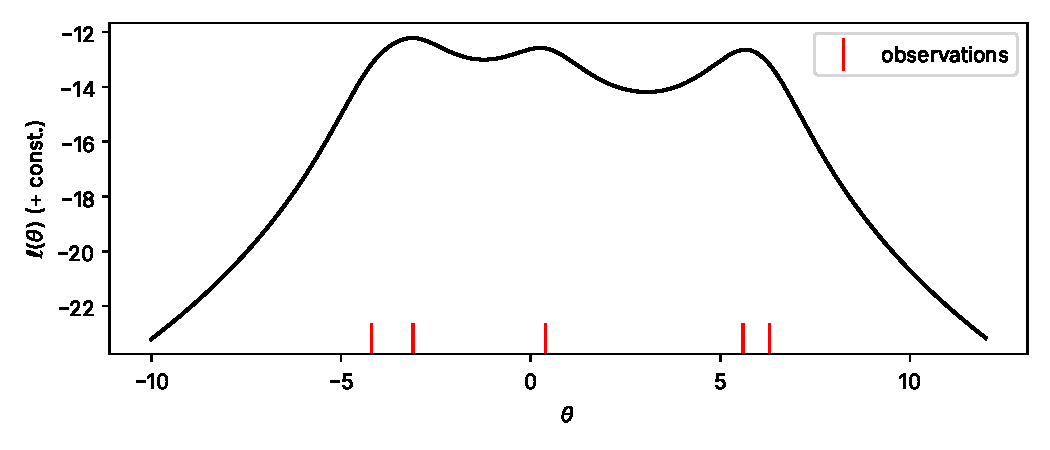
\includegraphics[width=0.8\textwidth]{figures/cauchy_ll.pdf}
\caption{Log-likelihood for a Cauchy sample of five observations. Data split into two clusters produce three local maxima (the two cluster centres and a compromise point between them); gradient methods converge to different peaks depending on the starting point. The global maximum is in the left cluster ($\hat\theta\approx-3.12$).}
\end{figure}

\section{Comments and Notes}

\begin{remark}[When the MLE Can Fail]
\begin{itemize}
  \item \textbf{Unbounded likelihood:} in a two-component normal mixture, if the mean of one component is set equal to an observation and its variance is sent to $0$, then $L\to\infty$; the global MLE\index{maximum likelihood estimator mle@maximum likelihood estimator (MLE)} is meaningless and one looks for ``the best local maximum'' (the EM algorithm).
  \item \textbf{Number of parameters growing with $n$} (the Neyman--Scott\index{neyman scott problem@Neyman--Scott problem} problem \cite{neyman-scott48}): if $X_{ij}\sim\Normal(\mu_i,\sigma^2)$, $j=1,2$, $i=1,\dots,n$, then $\hat\sigma^2\pto\sigma^2/2$: the MLE is inconsistent.
  \item \textbf{True parameter on the boundary:} asymptotic normality\index{asymptotic normality@asymptotic normality} breaks down (in Chapter~\ref{ch:lrt}, the counterpart of Wilks\index{wilks theorem@Wilks' theorem}' theorem is a mixture of chi-squares).
\end{itemize}
\end{remark}

\begin{remark}[Likelihood and the KL Divergence]
$\frac1n\ell(\theta)=\frac1n\sum\ln f(X_i;\theta)\asto\E_{\theta_0}\ln f(X;\theta)$ and
$\E_{\theta_0}\ln f(X;\theta_0)-\E_{\theta_0}\ln f(X;\theta)=\mathrm{KL}(f_{\theta_0}\|f_\theta)\ge0$. That is, the MLE minimises the KL divergence between the empirical distribution and the model. If the model is misspecified, the MLE converges to the member of the model closest in KL to the true distribution (the quasi-likelihood / QMLE interpretation).
\end{remark}

% --- CHAPTER SUMMARY ---
\section{Chapter Summary}
\begin{summary}
\begin{itemize}
  \item The MLE is the parameter value that maximises the likelihood. It is usually found as a root of the likelihood equation; when there is no closed form, numerical methods such as Newton--Raphson are used.
  \item Zehna's invariance principle (Theorem~\ref{thm:zehna}): even when $g$ is not one-to-one, $g(\hat\theta)$ is the MLE of $g(\theta)$ in the sense of the induced likelihood (Definition~\ref{def:induklenmis}).
  \item The MLE is a function of the sufficient statistic (Proposition~\ref{prop:mle-yeterli}). In a natural exponential family the likelihood equation becomes a moment equation: $\E_\eta T=T(\x)$ (Theorem~\ref{thm:ustel-mle}).
  \item The MLE does not always behave well. It may not exist, may not be unique, and the likelihood may have several local maxima (Cauchy). When the number of parameters grows with $n$, the MLE may even be inconsistent (Neyman--Scott).
\end{itemize}
\end{summary}
% --- END OF CHAPTER SUMMARY ---

\paragraph{Further reading.} \cite[Section~7.2]{casella}, \cite[Chapter~9]{wasserman}; for misbehaviour of the MLE\index{maximum likelihood estimator mle@maximum likelihood estimator (MLE)} see \cite[Chapter~6]{lehmann-casella}.

\section{Exercises}

\begin{exercise}\label{exr:11-1}
Let $X_i\iid\text{Poisson}(\lambda)$. Find the MLE of $\P(X=0)=e^{-\lambda}$ and compare it with the UMVUE in Example~\ref{ex:poisson-rb}. Which is biased?
\hfill\hyperref[coz:11-1]{\footnotesize$\rightarrow$\,Solution}
\end{exercise}

\begin{exercise}\label{exr:11-2}
Find the MLE of $(\mu,\lambda)$ for the shifted exponential distribution $f(x;\mu,\lambda)=\lambda e^{-\lambda(x-\mu)}\I\{x\ge\mu\}$. Compute the bias of $\hat\mu$ and propose an unbiased correction.
\hfill\hyperref[coz:11-2]{\footnotesize$\rightarrow$\,Solution}
\end{exercise}

\begin{exercise}\label{exr:11-3}
Under Hardy--Weinberg equilibrium the genotype probabilities are $(\theta^2,2\theta(1-\theta),(1-\theta)^2)$. Given observed counts $(n_1,n_2,n_3)$, show that $\hat\theta=\frac{2n_1+n_2}{2n}$ and compute $I_n(\theta)$.
\hfill\hyperref[coz:11-3]{\footnotesize$\rightarrow$\,Solution}
\end{exercise}

\begin{exercise}\label{exr:11-4}
Study the Neyman--Scott problem by simulation: show that for $n=1000$ pairs, $\hat\sigma^2$ approaches $\sigma^2/2$. Construct a consistent estimator by differencing ($X_{i1}-X_{i2}$).
\hfill\hyperref[coz:11-4]{\footnotesize$\rightarrow$\,Solution}
\end{exercise}

\chapterlinks{11}

\end{document}
